\subsection{Variational autoencoder}
Assume that the data $\mathbb{X}$ are generated by some random process, involving and unobserved continuous variable $\boldsymbol{z}$, which will be referenced as a latent variable or code. The objective is once again to find the PDF of the given data in a parametric form $p_{\bt}\left(\bx\right)$. One can choose approximative distribution in the form of
\begin{equation}
p_{\bt}\left(\bx\right) = \int p_{\bt}\left(\bx,  \boldsymbol{z}\right)\d{\boldsymbol{z}} =\int p_{\bt}\left(\bx\vert \boldsymbol{z}\right)p_{\bt}\left(\boldsymbol{z}\right)\d{\boldsymbol{z}},
\end{equation}
but such approximation is very expensive to compute or can be even intractable. Intractability of the $p_{\bt}\left(\bx\right)$ makes posterior PDF $p_{\bt}\left(\boldsymbol{z}\vert\bx\right)$ also intractable.
\subsubsection{Naive approach}
\subsubsection{Variational Bayes}
To solve this issue it is necessary to introduce further approximative posterior distribution $q_{\bphi}\left(\boldsymbol{z}\vert\bx\right) \approx p_{\bt}\left(\boldsymbol{z}\vert\bx\right)$ with parameters $\bphi$, preferably Gaussian. Standard terminology refers to the model $q_{\bphi}\left(\boldsymbol{z}\vert\bx\right)$ as a probabilistic \emph{encoder} and  $p_{\bt}\left(\bx\vert \boldsymbol{z}\right)$ is called a probabilistic \emph{decoder}.
For variational autoencoder (VAE) the idea is to use KL distance from $q_{\bphi}\left(\boldsymbol{z}\vert\bx\right)$ to $p_{\bt}\left(\boldsymbol{z}\vert \bx\right)$, yielding
\begin{equation}\label{eq:VAEloss}
\begin{split}
D_{\mathrm{KL}}\left(q_{\bphi}\left(\boldsymbol{z}\vert \bx \right) \Vert p_{\bt}\left(\boldsymbol{z}\vert \bx\right)\right) & = 
\int q_{\bphi}\left(\boldsymbol{z}\vert \bx \right) \log \frac{q_{\bphi}\left(\boldsymbol{z}\vert \bx \right)}{p_{\bt}\left(\boldsymbol{z}\vert \bx\right)} \d{\boldsymbol{z}} \\
& =  \int q_{\bphi}\left(\boldsymbol{z}\vert \bx \right) \log \frac{q_{\bphi}\left(\boldsymbol{z}\vert \bx \right)p_{\bt}\left(\bx\right)}{p_{\bt}\left(\bx \vert \boldsymbol{z}\right) p_{\bt}\left(\boldsymbol{z}\right)} \d{\boldsymbol{z}} \\
& = \log p_{\bt}\left(\boldsymbol{x}\right) +  \int q_{\bphi}\left(\boldsymbol{z}\vert \bx \right) \log \frac{q_{\bphi}\left(\boldsymbol{z}\vert \bx \right)}{p_{\bt}\left(\bx \vert \boldsymbol{z}\right)p_{\bt}\left(\boldsymbol{z}\right) } \d{\boldsymbol{z}} \\
& = \log p_{\bt}\left(\boldsymbol{x}\right) +  \mathbb{E}_{q_{\bphi}\left(\boldsymbol{z}\vert \bx \right)}\left[\log\frac{q_{\bphi}\left(\boldsymbol{z}\vert \bx \right)}{p_{\bt}\left(\boldsymbol{z}\right)} - \log p\left(\textbf{x}\vert \boldsymbol{z}\right)\right]\\
    & = \log p_{\bt}\left(\boldsymbol{x}\right) +\KL{q_{\bphi}\left(\boldsymbol{z}\vert \bx \right)}{p_{\bt}\left(\boldsymbol{z}\right)} -  \mathbb{E}_{q_{\bphi}\left(\boldsymbol{z}\vert \bx \right)}\left[\log p\left(\bx\vert \boldsymbol{z}\right)\right].
 \end{split}
\end{equation}
Using the last equality of \eqref{eq:VAEloss}, it is possible to rewrite the equation into its typical form
\begin{equation}
\log p_{\bt}\left(\bx\right) - D_{\mathrm{KL}}\left(q_{\bphi}\left(\boldsymbol{z}\vert \bx \right) \Vert p_{\bt}(\boldsymbol{z}\vert \bx)\right) = \underbrace{\mathbb{E}_{q_{\bphi}\left(\boldsymbol{z}\vert \bx \right)}\left[\log p_{\bt}(\bx\vert \boldsymbol{z}) \right] - D_{\mathrm{KL}}\left(q_{\bphi}\left(\boldsymbol{z}\vert\bx \right) \Vert p_{\bt}\left(\boldsymbol{z}\right)\right)}_{\text{= $L\left(\bt,\bphi; \bx\right)$}},
\end{equation}
where the right hand side is called \emph{variational} lower bound. There is no uniformity in terminology and thus one can also encounter the name evidence lower bound (ELBO). The first term of the right hand side is known as reconstruction loss and the second term is often called regularization term. As a KL distance is always non-negative, it holds
\begin{equation}
    \log p_{\bt}\left(\bx\right) \geq L\left(\bt,\bphi; \bx\right).
\end{equation}
The objective is to maximize the log-likelihood $\log p_{\bt}\left(\bx\right)$ which is equivalent to minimizing the negative log-likelihood and that is what will be used here. At this point we have a lower bound for one datapoint $\bx$, but we need to include all observations in the lower bound. Joint log-likelihood can be rewritten as a sum over the marginal log-likelihoods of individual observations $\log p_{\bt}\left(\bx_1,\bx_2,\dots,\bx_N\right)~=~\sum_{i=1}^N\log p_{\bt}\left(\bx_i\right)$ which completes all the building blocks needed to determine the optimization equation. This formulation provides one major advantage, which is that it is now possible to jointly optimize both the generative parameters $\bt$ and the variational parameters $\bphi$ as follows 
\begin{align}
   \widehat{\bt}, \widehat{\bphi} &= \argmin_{\bt,\bphi}-\sum_{i=1}^N\log p_{\bt}\left(\bx_i\right)\\
   &=\argmin_{\bt,\bphi}-\sum_{i=1}^N L\left(\bt,\bphi; \bx_i\right)\\
  &= \argmin_{\bt,\bphi}-\sum_{i=1}^N\mathbb{E}_{q_{\bphi}\left(\boldsymbol{z}\vert \bx_i \right)}\left[\log p_{\bt}(\bx_i\vert \boldsymbol{z}) \right] - D_{\mathrm{KL}}\left(q_{\bphi}\left(\boldsymbol{z}\vert\bx_i \right) \Vert p_{\bt}\left(\boldsymbol{z}\right)\right).\label{eq:VAEloss}
\end{align}
For a better understanding of the problem, a diagram of the VAE is shown in the Figure \ref{fig:VAE_architecture}.
 \begin{figure}[h]
	\centering
	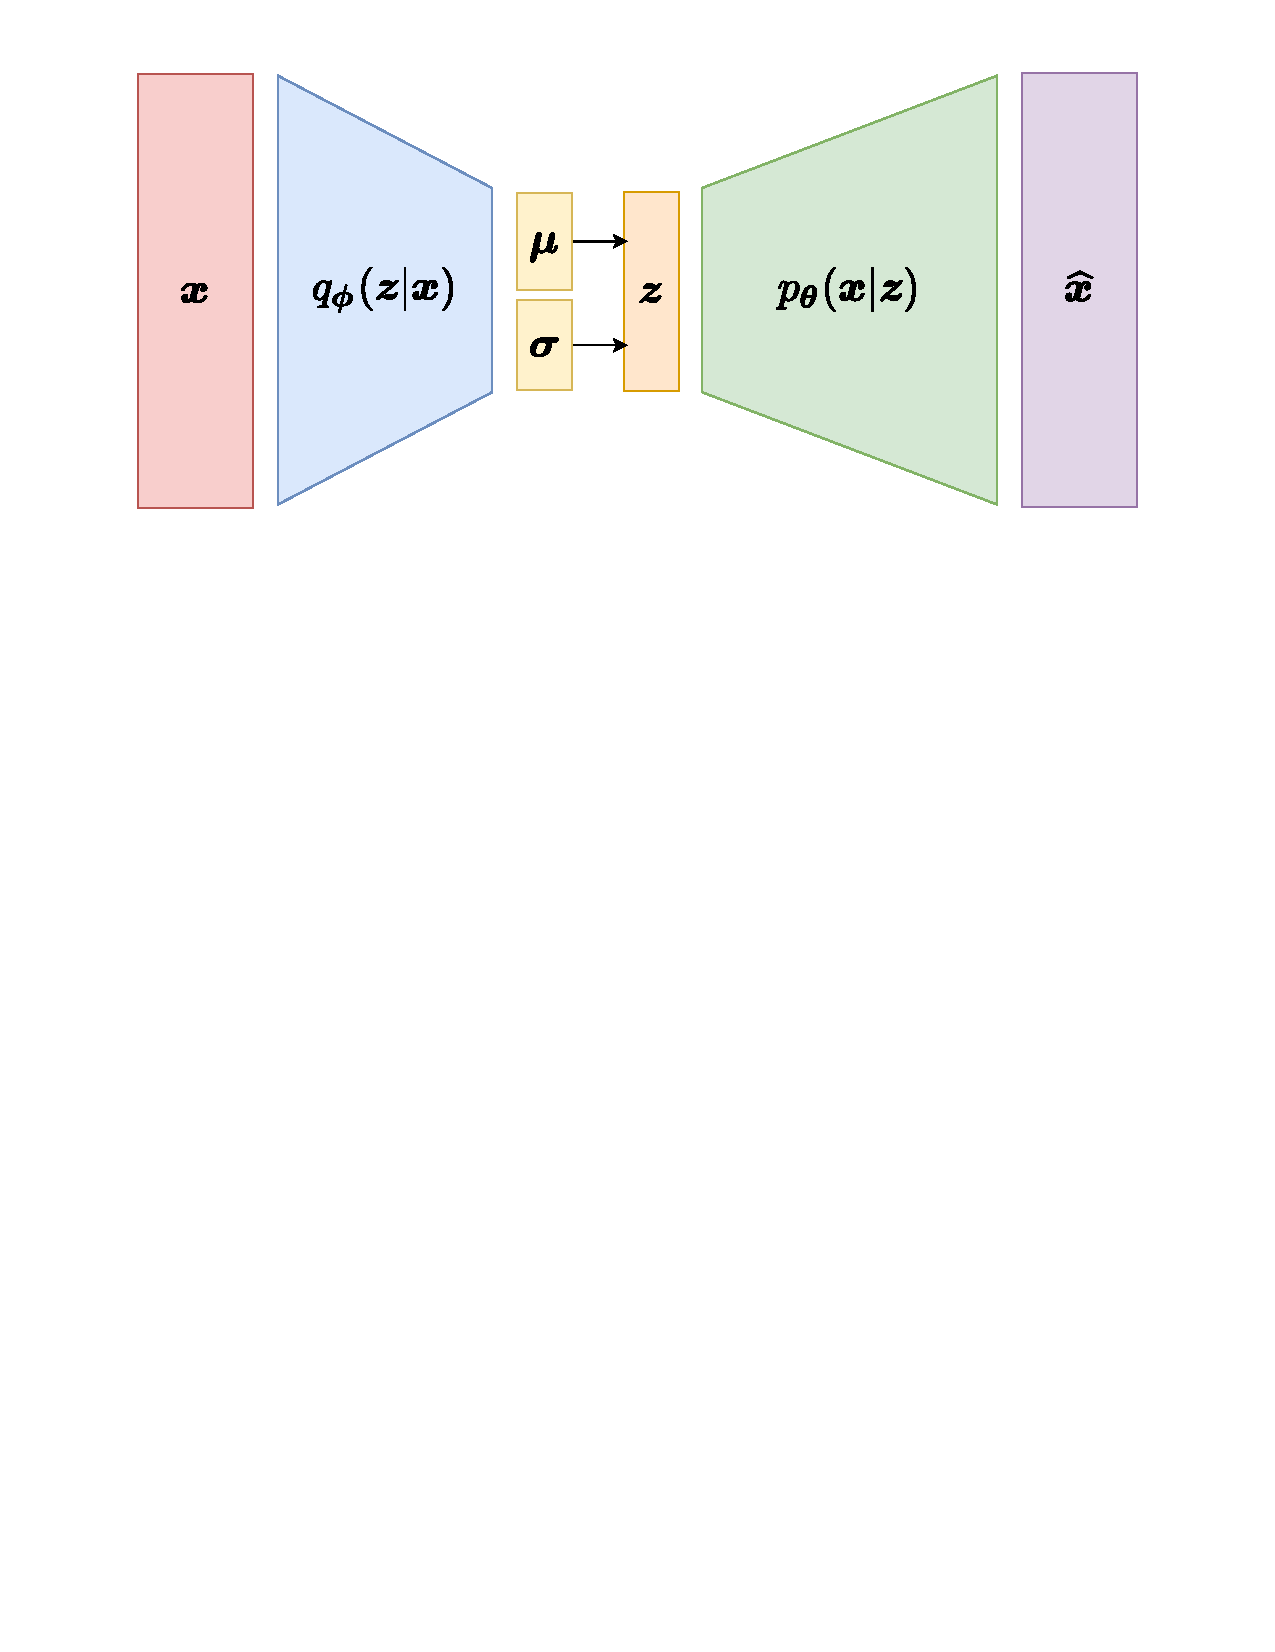
\includegraphics[width=\textwidth, trim={0 18cm 0 0}]{plots/Images/VAE_diagram.pdf}
	\caption{VAE diagram.}%
	\label{fig:VAE_architecture}%
\end{figure}

But before the actual optimization, it is essential to solve the stochastic node problem.   The key success of VAE is in the fact that \eqref{eq:VAEloss} can be efficiently computed using the \emph{reparameterization trick}
\begin{equation}
\boldsymbol{z}_{i,j} = \boldsymbol{\mu}_i + \boldsymbol{\sigma}_i\odot\boldsymbol{\varepsilon}_j ,
\end{equation}
where the symbol $\odot$ denotes Hadamard product, i.e. element-wise product and $\boldsymbol{\varepsilon} \sim \pazocal{N}\left(\boldsymbol{0},\mathbb{I} \right)$. 
Before applying the ELBO loss function to an optimization problem to backpropagate the gradient, it is necessary to make it differentiable by applying the so-called reparameterization trick to remove the stochastic sampling from the formation, and thus making it differentiable. 



\begin{equation}
q_{\bphi}\left(\boldsymbol{z}\vert \bx \right) = \pazocal{N}\left(\boldsymbol{z}; \boldsymbol{\mu},\boldsymbol{\sigma}  \right) ,
\end{equation}
můžeme parametry $\theta$ a $\phi$ minimalizovat zároveň a to následovně
\begin{equation}
\begin{split}
\hat{\theta},\hat{\phi} & = \argmin_{\theta, \phi}\sum_{i=1}^n\log p\left(x_i\right) \\
& = \argmin_{\theta, \phi}\left\lbrace  \mathbb{E}_q\left[\log p(\textbf{x}\vert \textbf{z}) \right] - D_{KL}\left(q\left(\textbf{z}\vert \textbf{x} \right) \Vert p(\textbf{z})\right)\right\rbrace . 
\end{split}
\end{equation}

\begin{equation}
\bx = f_{\bt}(\boldsymbol{z}) + \epsilon ,
\end{equation}
kde $\epsilon \sim \pazocal{N}\left(0,\sigma^2\cdot\mathbb{I}   \right)$ and  $f_{\theta}(\textbf{z})$ je neuronová síť.  Využijeme následující formu aproximace

Podle vztahu pro $\textbf{x}$ určíme distribuce $p\left(\textbf{x}\vert \textbf{z}\right)$ a $p\left(\textbf{z}\right)$ zvolíme jednoduše
\begin{equation}\label{VAE_latent}
\begin{split}
 p(\textbf{x}\vert \textbf{z}) &= \pazocal{N}\left(f_{\theta}(\textbf{z}),\sigma^2\cdot\mathbb{I} \right), \\
p(\textbf{z}) &= \pazocal{N}\left(0,\mathbb{I} \right).
\end{split}
\end{equation}

\subsubsection{Naivní přístup}
K nalezení $p(\textbf{x})$ je třeba najít parametry $\theta$ transformace $f_{\theta}(\textbf{z})$, proto zkusme sestavit věrohodnostní funkci $ \log p\left( \textbf{x}\right) = \log \prod_{i = 1}^n p\left(x_i \right) $  a minimalizovat 
\begin{equation}
\begin{split}
\hat{\theta} & = \argmin_{\theta} \sum_{i=1}^n \log p\left(x_{i} \right)\\
& =  \argmin_{\theta} \sum_{i=1}^n \log \int \pazocal{N}\left(f_{\theta}(z_j),\sigma^2 \right)\cdot\pazocal{N}\left(0,1 \right)    \dd z_j \\
& = \argmin_{\theta} \sum_{i=1}^n \ \log\sum_{j=1}^n \exp \left\lbrace -\frac{1}{2\sigma^2} \left(x_i - f_{\theta}(z_j)  \right)^2 \right\rbrace \cdot \exp \left\lbrace -\frac{z_j^2}{2} \right\rbrace .
\end{split}
\end{equation}
Integrace přes $\textbf{z}$ je nahrazena vzorkováním. Tento postup ovšem při minimalizaci nemusí konvergovat ke správným výsledkům.
\subsection{Variační Bayesova metoda}
Lepší metodou se ukazuje vzorkovat z podmíněné distribuce $q(\textbf{z}\vert \textbf{x})$ a využít ELBO

\begin{equation}
\begin{split}
D_{KL}\left(q\left(\textbf{z}\vert \textbf{x} \right) \Vert p(\textbf{z}\vert \textbf{x})\right) & = 
 \mathbb{E}_q\left[\log q(\textbf{z}\vert \textbf{x}) - \log p\left(\textbf{z}\vert \textbf{x} \right)\right] \\
 & =  \mathbb{E}_q\left[\log q(\textbf{z}\vert \textbf{x}) - \log p(\textbf{x}\vert \textbf{z}) - \log p(\textbf{z}) + \log p(\textbf{x})   \right] .
 \end{split}
\end{equation}
Tuto rovnici můžeme přepsat pomocí KL--divergence 
\begin{equation}
\log p(\textbf{x}) - D_{KL}\left(q\left(\textbf{z}\vert \textbf{x} \right) \Vert p(\textbf{z}\vert \textbf{x})\right) = \mathbb{E}_q\left[\log p(\textbf{x}\vert \textbf{z}) \right] - D_{KL}\left(q\left(\textbf{z}\vert\textbf{x} \right) \Vert p(\textbf{z})\right) ,
\end{equation}
kde pravá strana této rovnice je lower bound objektu $\log p(\textbf{x})$.
Jestliže vybereme parametrickou formu distribuce
\begin{equation}
q\left(\textbf{z}\vert \textbf{x} \right) = \pazocal{N}\left(\mu_{\phi}(\textbf{x}), \diag\left(\sigma^2_{\phi}(\textbf{x})\right) \right) ,
\end{equation}
můžeme parametry $\theta$ a $\phi$ minimalizovat zároveň a to následovně
\begin{equation}
\begin{split}
\hat{\theta},\hat{\phi} & = \argmin_{\theta, \phi}\sum_{i=1}^n\log p\left(x_i\right) \\
& = \argmin_{\theta, \phi}\left\lbrace  \mathbb{E}_q\left[\log p(\textbf{x}\vert \textbf{z}) \right] - D_{KL}\left(q\left(\textbf{z}\vert \textbf{x} \right) \Vert p(\textbf{z})\right)\right\rbrace . 
\end{split}
\end{equation}
V metodě variačního autoencoderu jsou nezbytné následující dva fakty.
\begin{enumerate}
\item Trik v \textbf{reparametrizaci}
\begin{equation}
\textbf{z} = \mu_{\phi}(\textbf{x}) + \sigma_{\phi}(\textbf{x})\odot\epsilon ,
\end{equation}
kde $\odot$ značí Hadamardův součin, čili součin po složkách.
To můžeme zapsat jednodušeji takto
\begin{equation}
z_i = \mu_{\phi}(x_i) + \sigma_{\phi}(x_i)\cdot\epsilon_i .
\end{equation}
Nejedná se v podstatě o nic jiného, než o transformaci náhodné veličiny.
\item  KL--divergence dvou Gaussovských distribucí má analytické řešení a nabude tvaru
\begin{equation}
\begin{split}
 D_{KL}\left(q\left(\textbf{z}\vert \textbf{x} \right) \Vert p(\textbf{z})\right) & = \frac{1}{2}\left[\tr\left(\diag\left(\sigma_{\phi}^2(\textbf{x})\right)\right) - \mu_{\phi}\tran(\textbf{x})\mu_{\phi}(\textbf{x}) - k - \log\det \diag\left(\sigma_{\phi}^2(\textbf{x})   \right)\right] \\
 & = \frac{1}{2}\left[\sum_{l = 1}^k(\sigma_{\phi}^2(\textbf{x})) -\mu_\phi\tran(\textbf{x})\mu_{\phi}(\textbf{x}) - k - \sum_{l = 1}^k\log\sigma_{\phi}^2(\textbf{x})    \right],
\end{split}
\end{equation}
kde $k$ značí dimenzi Gaussova rozdělení. 
\end{enumerate}

Kdybychom totiž nevybrali aproximační distribuce Gaussovské, nemohli bychom tímto způsobem $\hat{\theta},\hat{\phi}$ určit. Díky těmto dvěma faktům tak získáme konečný tvar odhadu parametrů

\begin{multline}\label{řešení_VAE}
 \hat{\theta},\hat{\phi}   = \argmin_{\theta, \phi}\sum_{i = 1}^n\sum_{j = 1}^p \left[ x_i - f_\theta \left(\mu_{\phi}(x_i) + \sigma_{\phi}(x_i)\cdot\epsilon_{i,j}  \right)        \right] ^2  \\ -   \frac{1}{2}\left[\sum_{l = 1}^k(\sigma^2_{\phi}(x_i)) -\mu_{\phi}\tran(x_i)\mu_{\phi}(x_i) - k - \sum_{l = 1}^k\log\sigma^2_{\phi}(x_i)   \right] .
\end{multline}

